\section{Аналитическая часть}

\subsection{Постановка задачи}
Результатом работы должна стать программа для загрузки файлов по протоколу Bittorrent, удовлетворяющая следующим требованиям:
\begin{itemize}
	\item поддерживать файлы расширения .torrent;
	
	\item поддерживать функцию загрузки данных как от сервера, так и от других клиентов;
	
	\item обладать графическим интерфейсом для удобства выполнения действий и просмотра текущей информации по состоянию загрузки.
	
\end{itemize}
%
Первостепенной задачей для дальнейшей разработки является изучения устройства выбранного протокола.
%
 \newline

\subsection{Принцип работы протокола}
Bittorrent -- P2P протокол для кооперативного обмена файлами через интернет \cite{doc,wiki}. 

В данном протоколе выделены две роли:
\begin{enumerate}
	\item \textbf{пир} (клиент) хранит файлы и производит обмен их частями с другими пирами;
	
	\item \textbf{трекер} (сервер) хранит таблицу файлов и список пиров, имеющих данный файл в распоряжении. \newline
\end{enumerate}

Пир, желающий получить файл должен обладать \textbf{.torrent файлом}, с помощью которого он может обратиться к серверу. Сервер предоставляет адреса клиентов, обладающих запрашиваемыми файлами после чего начинается их загрузка. Передача осуществляется частями (\textbf{pieces}), каждый torrent-клиент, скачивая эти части, в то же время отдаёт их другим клиентам, что снижает нагрузку на каждого отдельного клиента (Рисунок \ref{fig100:image}) \cite{wiki,understand}. 

\begin{figure}[h!]
	\begin{center}
		{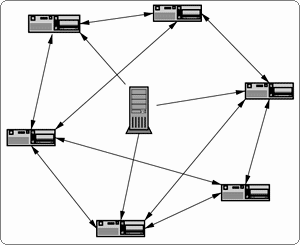
\includegraphics[scale = 0.7]{img/torrent.png}}
		\caption{Схема взаимодействия клиентов и сервера}
		\label{fig100:image}
	\end{center}
\end{figure}

\subsection{Структура .torrent файла}
Как было отмечено выше, первым шагом в начале загрузки является получение и парсинг файла специального расширения .torrent.

Для кодирования данных в .torrent-файлах используется формат Bencode. Само содержимое -- ассоциативный массив с полями:
\begin{itemize}
	\item \textbf{info} -- вложенный ассоциативный массив который описывает файлы, передаваемые торрентом;
	
	\item \textbf{announce} -- URL трекера;
	
	\item \textbf{announce-list} -- список трекеров, если их несколько, в Bencode-виде — список списков;
	
	\item \textbf{creation date} -- дата создания;
	
	\item \textbf{comment} -- текстовое описание торрента;
	
	\item \textbf{created by} -- автор торрента. \\
\end{itemize}

info и announce являются обязательными полями, всё остальные — опционально. Первый в свою очередь состоит из:
\begin{itemize}
	\item \textbf{piece length} -- размер одного куска;
	
	\item \textbf{pieces} -- конкатенация SHA1-хешей каждого куска (каждый хеш - 20 байт);
	
	\item \textbf{name} -- имя файла (если файл один);
	
	\item \textbf{length} -- содержит длину файла (если файл один);
	
	\item \textbf{files} -- если файлов несколько, то содержит список ассоциативных массивов (с указанием length и path). \\
\end{itemize}

Данная информация используется на всём протяжении загрузки файла и его последующей раздаче. \newline

\subsection{Взаимодействие клиента и сервера}
Чтобы перейти к загрузке файла клиент должен получить список пиров у трекера. Для этого он должен отправить GET-запрос, называемый \textbf{анонсом}, по адресу announce по пути /announce. 

После данного действия трекер узнаёт о наличии нового клиента и может выдать его адрес другим клиентам. Указываются следующие URL-параметры.

\begin{itemize}
	\item \textbf{info\_hash} -- SHA1-хеш словаря info. Используется для поиска файла в таблице трекера, то есть фактически является его уникальным идентификатором.
	
	\item \textbf{peer\_id} -- уникальный ID клиента. Имеет вид \textit{-<2-символьный id><номер версии из 4 цифр>-<12 случайных цифр>}. Такой код может быть сгенерирован клиентом самостоятельно, так как вероятность коллизии с другими клиентами крайне мала (число возможных вариантов peer\_id одной версии превышает количество IPv4 адресов более чем в 200 раз).
	
	\item \textbf{uploaded}, \textbf{downloaded}, \textbf{left} -- количество отправленных, загруженных и незагруженных байтов.
	
	\item \textbf{port} -- TCP-порт, прослушиваемый клиентом. Общепринятыми значениями являются 6881-6889.
	
	\item \textbf{compact} -- признак того, принимает ли клиент компактный список пиров. \\
	
\end{itemize}

В случае, если запрос прошёл успешно и по info\_hash был найден необходимый torrent, трекер посылает ответ (также по протоколу HTTP). В его теле содержится следующие поля в формате Bencode:
\begin{itemize}
	\item \textbf{interval} -- интервал в секундах до того, как клиент должен сделать новый запрос к трекеру;
	
	\item \textbf{peers} -- список пиров. В случае, если в запросе compact был равен 1, в ответе будет список будет заменён бинарной строкой, которую потребуется разбить на группы по 6 байт для выделения IPv4 адреса и порта каждого пира. \\
\end{itemize}

Подобные запросы будут повторяться раз в interval секунд для поддержания сервера в курсе актуального состояния загрузки и для получения новых адресов пиров. \newline

\subsection{Структура сообщений}
Протокол BitTorrent определяет следующий способ обмена сообщениями для клиентов, его особенности:
\begin{itemize}
	\item использует стек TCP/IP;
	
	\item файл передаётся по кускам фиксированного размера, не в порядке их следования в файле. \\
\end{itemize}

Определена следующая структура p2p сообщения:
\begin{enumerate}
	\item \textbf{длина}, Len (4Б) -- размер типа и полезной нагрузки сообщения;
	
	\item \textbf{тип}, ID (1Б) определяет вид сообщения и способ его обработки;
	
	\item \textbf{полезная нагрузка}, Payload (0 - 32КБ) содержит передаваемую информацию. \\
\end{enumerate}

Различаются следующие типы сообщений.
\begin{itemize}
	\item \textbf{handshake}: <len=49+X><info\_hash><peer\_id>. Сообщение рукопожатия. Отправляется один раз в начале обмена информацией. Содержит название протокола, хеш код файла и собственный id.
	
	\item \textbf{keep-alive}: <len=0000>. Содержит только нулевую длину. Используется чтобы один из пиров не закрыл соединение по истечению времени без сообщений.
	
	\item \textbf{choke}: <len=0001><id=0>. Используется для запрета другому пиру отправки сообщений до момента посылки ему unchoke.
	
	\item \textbf{unchoke}: <len=0001><id=1>.

	\item \textbf{interested}: <len=0001><id=2>. Состояние говорит о том, что пир заинтересован в получении фрагментов.
	
	\item \textbf{not interested}: <len=0001><id=3>. Обратно interested.
	
	\item \textbf{have}: <len=0005><id=4>. Сообщает о появлении в своём распоряжении куска с указанным индексом.
	
	\item \textbf{bitfield}: <len=0001+X><id=5>. Содержит в себе карту битов, описывающую статус всех кусков файла.
	
	\item \textbf{request}: <len=0013><id=6>. Используется для запроса блока байт размером length, начинающимся с позиции begin из куска с номером index.
	
	\item \textbf{piece}: <len=0009+X><id=7>. Сообщение содержит в себе блок байт block по формату, описанному в request. \newline
\end{itemize}

\subsection{Взаимодействие клиентов}
Первым шагом после получения адреса пира требуется выполнения "рукопожатия" (handshake). Он нужен для обмена id и проверкой совпадения протоколов и контрольного хеша файла. В случае неудачного рукопожатия TCP соединение разрывается.

После рукопожатия устанавливается состояние Choked. Для выхода из него сразу отправляется сообщение Interested для перехода к обмену.

В первую очередь после взаимной заинтересованности пиры обмениваться информацией о наличии кусков с помощью сообщения bitfield. Это требуется для определения отсутствующих кусков, которые можно запросить у данного пира. 

В тот момент, когда клиент может запросить кусок (т.е. не находится уже в состоянии загрузки с данным пиром, не является choked и not interested), он выбирает блок для запроса у данного пира. Приоритет выбора следующий \cite{survey}:
\begin{enumerate}
	\item блоки, для которых истекло время ожидания;
	
	\item блоки из неполностью загруженных кусков;
	
	\item блоки из наиболее редких кусков. \\
\end{enumerate}

Блоки будут отсутствовать во всех перечисленных категориях только в случае, если загрузка почти полностью завершена. Такая ситуация называется \textbf{end-game}. В этом случае в качестве очередных блоков для запроса выбираются уже загружаемые блоки.

После получения блока (сообщения piece), он записывается с указанным смещением в нужный кусок. По окончанию загрузки куска подсчитывается его контрольная сумма и сравнивается с той, которая изначально хранилась в torrent файле. Если они совпали, кусок помечается загруженным и сохраняется в загружаемый файл, а всем хостам без данного куска отправляется сообщение Have с его номером.

Файл считается загруженным полностью кода скачены и проверены все его куски. \newline

\subsection*{Вывод}
Результатом аналитического раздела стал анализ устройства протокола BitTorrent, алгоритма взаимодействия с сервером и другими пирами.